\documentclass{standalone}
\usepackage{pgfplots}
\usepackage{lmodern}
\usepackage{pgf-pie}
\pgfplotsset{compat=1.18}

\definecolor{coal}{HTML}{526D82}
\definecolor{oil}{HTML}{9DB2BF}
\definecolor{ng}{HTML}{DDE6ED}
\definecolor{nuclear}{HTML}{0078D4}
\definecolor{hydro}{HTML}{1A5319}
\definecolor{bio}{HTML}{508D4E}
\definecolor{wind}{HTML}{80AF81}
\definecolor{solar}{HTML}{D6EFD8}

\begin{document}
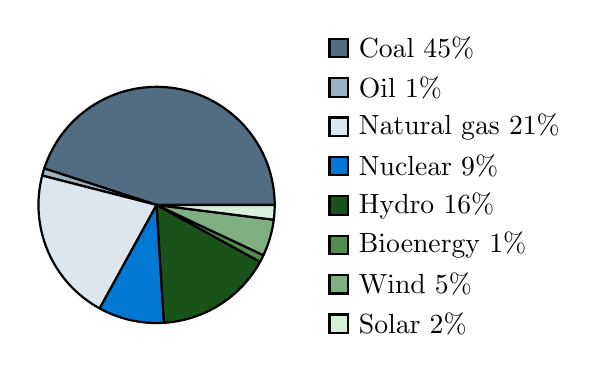
\begin{tikzpicture}
	\pie[
		radius=1.5, text=legend,
		hide number,
		color={coal, oil, ng, nuclear, hydro, bio, wind, solar}
	]
	{45/Coal 45\%, 1/Oil 1\%, 21/Natural gas 21\%, 9/Nuclear 9\%, 16/Hydro 16\%, 1/Bioenergy 1\%, 5/Wind 5\%, 2/Solar 2\%}
\end{tikzpicture}
\end{document}